\tikzset{
	ppblock/.style={
		rectangle,
		minimum size=6mm,
		very thick,
		draw=black!50,
		text centered,
		font=\ttfamily,
		minimum width=8em,
		minimum height=6mm,
		top color=white,
	},
	%
	figure/.style={
		rectangle,
		rectangle split,
		rectangle split parts=2,
		very thick,
		draw=black!50,
		text centered,
		append after command={
			\pgfextra
			\fill[top color=#1, bottom color=#1]
			(\tikzlastnode.one west) 
			[rounded corners] |- (\tikzlastnode.north) -| (\tikzlastnode.one east) 
			[sharp corners]   |- (\tikzlastnode.one split) -| cycle;
			\fill[top color=white, bottom color=#1]
			(\tikzlastnode.two west) 
			[rounded corners] |- (\tikzlastnode.south) -| (\tikzlastnode.two east)  
			[sharp corners]   |- (\tikzlastnode.one split) -| cycle;
			\endpgfextra
		},
	},
    splitted/.style={
        rectangle,
        rectangle split,
        rectangle split horizontal,
        rectangle split parts=2,
        very thick,
        draw=black!50,
        text centered,
        append after command={
            \pgfextra
            \fill[top color=white, bottom color=#1]
            (\tikzlastnode.south)
            [rounded corners] -| (\tikzlastnode.west) |- (\tikzlastnode.one north)
            [sharp corners]   -| (\tikzlastnode.one split) |- cycle;
            \fill[top color=white, bottom color=#1]
            (\tikzlastnode.two south)
            [rounded corners] -| (\tikzlastnode.east) |- (\tikzlastnode.north)
            [sharp corners]   -| (\tikzlastnode.one split) |- cycle;
            \endpgfextra
        },
    },
	%
	static/.style={ppblock, bottom color={black!20}},
	nonterminal/.style={ppblock, bottom color={blue!30}},
	terminal/.style={ppblock, bottom color={green!20}},
	algorithm/.style={ppblock, bottom color={yellow!50}},
	error/.style={ppblock, bottom color={red!20}},
	type/.style={ppblock, bottom color={red!20}},
	loss/.style={ppblock, dashed, bottom color={black!20}, font=\itshape},
	%
	tiny/.style={
		rounded rectangle,
		very thick,
		draw=black!50,
		top color=white,
		bottom color=red!20,
        text centered,
		font=\ttfamily,
	},
    operator/.style = {
        circle,
        scale=0.6,
        draw=black!50,
        top color=white,
        bottom color=red!20,
        font=\boldmath,
    },
	%
	skip loop/.style={to path={-- ++(0,#1) -| (\tikztotarget)}}
}

\begin{tikzpicture}[
>=stealth',thick,
tip/.style={->,shorten >=0.007pt},
every node/.style={scale=0.7},
]

\matrix (table) [matrix of nodes, column sep=6mm, row sep=6mm, align=center] {
    \node (false)        [figure={green!20}]      {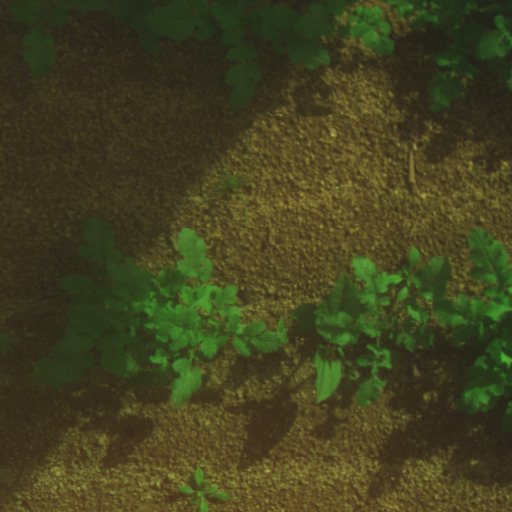
\includegraphics[width=4cm]{img/leaf/airphen-false} \nodepart{second} {\faShare*} Pre-Processing}; &
    \node (index)        [figure={blue!30}]      {\includegraphics[width=4cm]{img/leaf/airphen-index} \nodepart{second} {\faPagelines} Deep-Indices}; &
    \node (watershed)    [figure={blue!30}]      {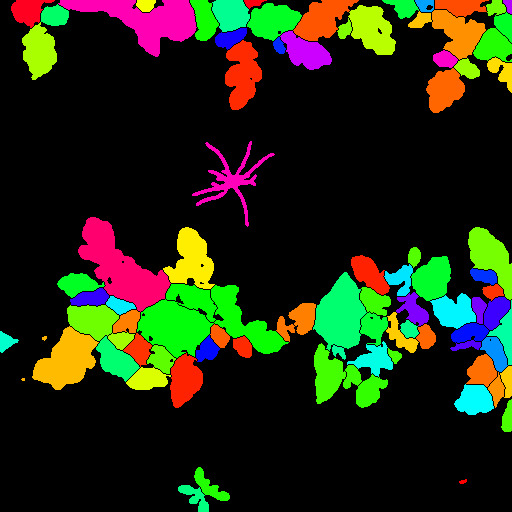
\includegraphics[width=4cm]{img/leaf/airphen-watershed} \nodepart{second} {\faLeaf} Deep-Leaves}; &
    \node (fv)    [nonterminal,rotate=90,xshift=16mm]      {{\faBolt} Optimization \\ {\faCalculator} Feature Extraction \\ {\faChartPie} And Data-Mining}; &
    %\node (cl)    [nonterminal,rotate=90,xshift=16mm]      {Classification}; &
    \node (map)    [figure={green!20}]      { \includegraphics[width=4cm]{img/conclusion/airphen-crop-weed-map} \nodepart{second} {\faSearch} Classification}; \\
};

\draw[->] (false) to (index);
\draw[->] (index) to (watershed);
\draw[->] (watershed) to (fv);
\draw[->] (fv) to (map);

\end{tikzpicture}